\chapter{Функции и графики}\markright{Глава 13}
\begin{definition}\term{Функция} (\emph{function}) — соответствие, которое каждому \(x\) из области определения ставит в соответствие ровно одно значение \(f (x)\).\end{definition}
\begin{definition}\term{Область определения} (\emph{domain}) функции — множество всех допустимых значений аргумента \(x\).\end{definition}
\begin{definition}\term{Область значений} (\emph{range; image}) функции — множество всех значений \(f(x)\), которые она принимает.\end{definition}
\begin{definition}\term{График функции} (\emph{graph of a function}) \(f\) — множество точек \((x;f(x))\) при всех \(x\) из её области определения.\end{definition}
\begin{definition}\term{Нули функции} (\emph{zeros of a function}) — значения \(x\) из области определения, для которых \(f(x)=0\).\end{definition}
\begin{definition}\term{Строгое возрастание} (\emph{strict increase}) функции \(f\) на промежутке \(I\) означает: для любых \(x_1,x_2\in I\) из \(x_1<x_2\) следует \(f(x_1)<f(x_2)\).\end{definition}
\begin{definition}\term{Строгое убывание} (\emph{strict decrease}) функции \(f\) на промежутке \(I\) означает: для любых \(x_1,x_2\in I\) из \(x_1<x_2\) следует \(f(x_1)>f(x_2)\).\end{definition}
В этом сборнике слова «возрастает» и «убывает» означают строгую монотонность.
\begin{definition}\term{Неубывающая функция} (\emph{nondecreasing function}) на промежутке \(I\) — функция, для которой при любых \(x_1,x_2\in I\) из \(x_1<x_2\) следует \(f(x_1)\le f(x_2)\). Это более слабое условие, чем строгое возрастание.\end{definition}
\begin{definition}\term{Чётная функция} (\emph{even function}) — функция с симметричной относительно нуля областью определения, для которой \(f(-x)=f(x)\) при всех допустимых \(x\). Симметричность области означает, что вместе с \(x\) она содержит \(-x\).\end{definition}
\begin{definition}\term{Нечётная функция} (\emph{odd function}) — функция с симметричной относительно нуля областью определения, для которой \(f(-x)=-f(x)\) при всех допустимых \(x\).\end{definition}
\section*{Графики и преобразования}
\(y = f (x - a)\) при \(a > 0\) сдвигает график вправо на \(a\). \(y = f (x) + b\) при \(b > 0\) сдвигает его вверх на \(b\).\par
\(y = - f (x)\) отражает график относительно горизонтальной оси. \(y = f (- x)\) отражает его относительно вертикальной оси.\par
Чтобы найти пересечения двух графиков, реши \(f (x) = g (x)\), затем вычисли \(y\) для каждого найденного \(x\).\par
\begin{definition}\term{Композиция} (\emph{composition}) функций \(f\) и \(g\), обозначаемая \(f(g(x))\), — функция, для вычисления которой сначала находят \(g(x)\), затем подставляют результат в \(f\). Аргумент \(x\) должен принадлежать области определения \(g\), а значение \(g(x)\) — области определения \(f\).\end{definition}
{\small\textit{Пример: \(y = (x - 2)^{2} + 1\) имеет вершину \((2;\allowbreak 1)\) и область значений \([1;\allowbreak + \infty )\).}}\par

\section*{Отображения и обратные функции}
\begin{definition}\term{Отображение} (mapping) \(f:X\to Y\) — правило, которое каждому элементу \(x\) множества \(X\) сопоставляет ровно один элемент \(f(x)\) множества \(Y\). Для числовых множеств это привычная числовая функция.\end{definition}
\begin{definition}\term{Множество назначения} (codomain) отображения \(f:X\to Y\) — указанное множество \(Y\), в котором лежат результаты отображения. Оно может быть больше области значений.\end{definition}
\begin{definition}\term{Образ множества} (image) \(X\) при отображении \(f\) — множество всех полученных значений: \(f(X)=\{f(x):x\in X\}\). Поэтому \(f(X)\subseteq Y\).\end{definition}
\begin{definition}\term{Инъекция} (injection) — отображение \(f:X\to Y\), для которого из \(f(x_1)=f(x_2)\) следует \(x_1=x_2\). Различные аргументы имеют различные образы.\end{definition}
\begin{definition}\term{Сюръекция} (surjection) — отображение \(f:X\to Y\), для которого каждый \(y\in Y\) равен \(f(x)\) хотя бы при одном \(x\in X\). Иначе говоря, \(f(X)=Y\).\end{definition}
\begin{definition}\term{Биекция} (bijection) — отображение, являющееся одновременно инъекцией и сюръекцией. Каждый элемент множества назначения имеет ровно один прообраз.\end{definition}
\begin{definition}\term{Обратное отображение} (inverse mapping) к биекции \(f:X\to Y\) — отображение \(f^{-1}:Y\to X\), которое каждому \(y\) сопоставляет единственный \(x\), для которого \(f(x)=y\). Запись \(f^{-1}\) здесь не означает \(\frac{1}{f}\).\end{definition}
\begin{theorem}[Существование обратного отображения]
Отображение \(f:X\to Y\) имеет обратное отображение \(g:Y\to X\), удовлетворяющее \(g(f(x))=x\) для всех \(x\in X\) и \(f(g(y))=y\) для всех \(y\in Y\), тогда и только тогда, когда \(f\) — биекция.
\end{theorem}
\par\addvspace{5pt}\begin{lrbox}{\CatFlowBox}\begin{minipage}[t]{\linewidth}
\setlength{\parskip}{5pt}\setlength{\columnsep}{4.5mm}\setlength{\intextsep}{0pt}
\begin{wrapfigure}[12]{r}{54mm}

\includegraphics[width=54mm,height=58mm,keepaspectratio]{images/unique/art-25.png}
\end{wrapfigure}
\textit{Доказательство.} Если \(f\) — биекция, сюръективность обеспечивает существование прообраза каждого \(y\), а инъективность — его единственность. Выбирая этот прообраз, получаем \(g=f^{-1}\) и оба равенства. Обратно, пусть оба равенства выполнены. Из \(f(x_1)=f(x_2)\) после применения \(g\) следует \(x_1=x_2\), поэтому \(f\) инъективно. Для каждого \(y\in Y\) равенство \(f(g(y))=y\) даёт прообраз, поэтому \(f\) сюръективно.\hfill\(\blacksquare\)

Важен выбор множества назначения: \(x\mapsto x^2\) из \(\mathbb R\) в \(\mathbb R\) не является сюръекцией, а из \(\mathbb R\) в \([0;+\infty)\) является. Оба отображения неинъективны. Ограничив аргументы множеством \([0;+\infty)\), получаем биекцию \(x\mapsto x^2\) на \([0;+\infty)\), обратную функции \(y\mapsto\sqrt y\).
\par\WFclear\end{minipage}\end{lrbox}%
\ifdim\dimexpr\ht\CatFlowBox+\dp\CatFlowBox\relax<64mm\dp\CatFlowBox=\dimexpr64mm-\ht\CatFlowBox\relax\fi%
\noindent\usebox{\CatFlowBox}\par\addvspace{5pt}
\begin{example}
Функция \(f(x)=3x+2\) задаёт биекцию \(\mathbb R\to\mathbb R\). Из \(y=3x+2\) находим \(x=\frac{y-2}{3}\), поэтому \(f^{-1}(y)=\frac{y-2}{3}\). Проверка: \(f^{-1}(f(x))=x\) и \(f(f^{-1}(y))=y\). Графики обратных числовых функций симметричны относительно прямой \(y=x\): точке \((x;y)\) первого графика соответствует точка \((y;x)\) второго.
\end{example}
\begin{definition}\term{Композиция отображений} (composition) \(g:X\to Y\) и \(f:Y\to Z\) — отображение \(f\circ g:X\to Z\), заданное правилом \((f\circ g)(x)=f(g(x))\). Сначала применяют \(g\), затем \(f\).\end{definition}
Если формулы заданы на своих естественных областях, область определения \(f\circ g\) состоит из тех \(x\) из области определения \(g\), для которых \(g(x)\) входит в область определения \(f\). Например, при \(f(u)=\sqrt u\), \(g(x)=2x-1\) композиция \(f(g(x))=\sqrt{2x-1}\) определена при \(x\ge\frac12\), а \(g(f(x))=2\sqrt x-1\) — при \(x\ge0\).

\par\noindent\begin{minipage}{\linewidth}\section*{Графики}
\begin{center}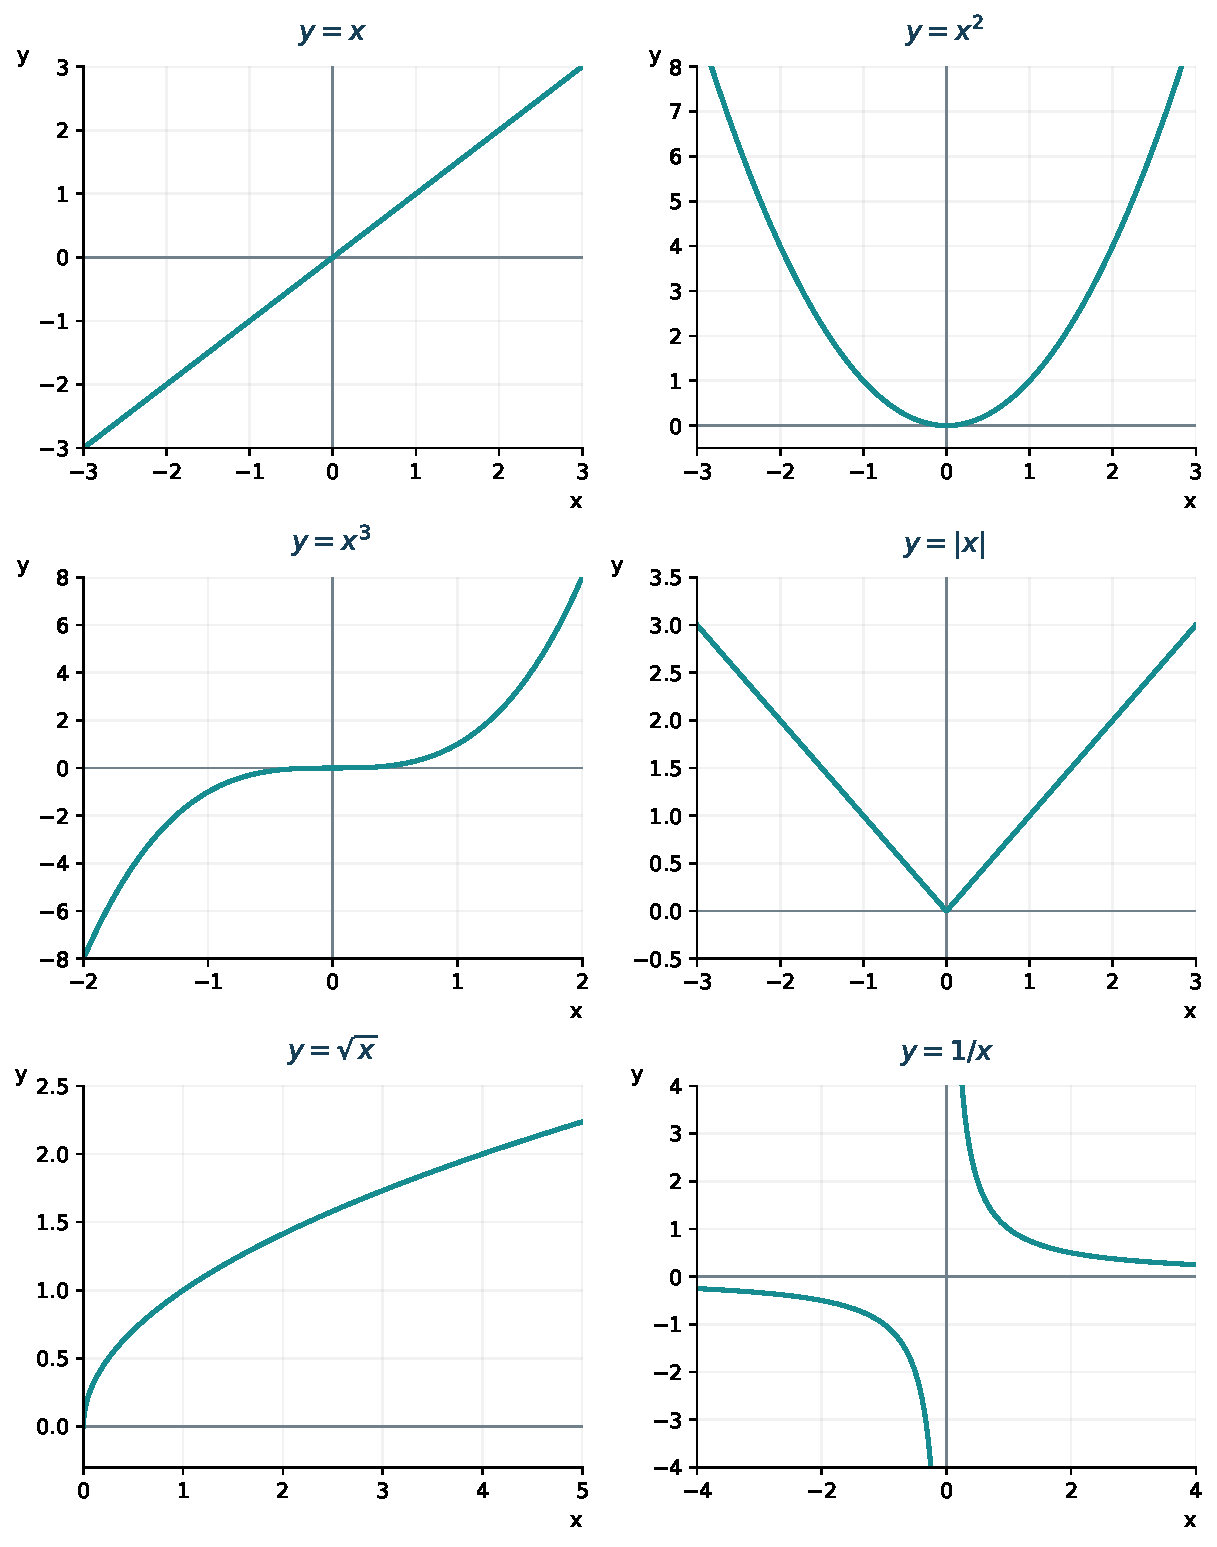
\includegraphics[width=\textwidth,height=.70\textheight,keepaspectratio]{images/atlas-algebra.pdf}\par\small Базовые алгебраические функции\end{center}\end{minipage}\par
\Needspace{7\baselineskip}\section*{Задачи}
\begingroup\setlength{\parskip}{3pt}
\noindent\begin{minipage}[t]{\linewidth}\textbf{13.1.} Для \(f (x) = 2 x - 3\) найди \(f (- 2),\allowbreak f (0),\allowbreak f (3)\).\par\end{minipage}\par
\noindent\begin{minipage}[t]{\linewidth}\textbf{13.2.} Найди область определения \(f (x) = \dfrac{1}{x - 4}\).\par\end{minipage}\par
\noindent\begin{minipage}[t]{\linewidth}\textbf{13.3.} Найди область определения \(f (x) = \sqrt{x + 3}\).\par\end{minipage}\par
\noindent\begin{minipage}[t]{\linewidth}\textbf{13.4.} Найди нули \(f (x) = x^{2} - 4\).\par\end{minipage}\par
\par\addvspace{5pt}\begin{lrbox}{\CatFlowBox}\begin{minipage}[t]{\linewidth}
\setlength{\parskip}{5pt}\setlength{\columnsep}{4.5mm}\setlength{\intextsep}{0pt}
\begin{wrapfigure}[12]{l}{54mm}

\includegraphics[width=54mm,height=58mm,keepaspectratio]{images/unique/art-38.png}
\end{wrapfigure}
\textbf{13.5.} Где \(f (x) = 3 x - 6\) положительна?\par

\textbf{13.6.} Построй \(y = 2 x + 1\) и найди пересечения с осями.\par

\textbf{13.7.} Построй \(y = (x - 2)^{2} - 1\). Укажи вершину.\par

\textbf{13.8.} Укажи промежутки убывания и возрастания \(y = x^{2}\).\par

\textbf{13.9.} Определи чётность \(f (x) = x^{3}\) и \(g (x) = x^{2} + 1\).\par

\textbf{13.10.} При \(f (x) = x^{2}\) и \(g (x) = x + 1\) найди \(f (g (x))\) и \(g (f (x))\).\par

\textbf{13.11.} Найди область значений \(y = (x - 1)^{2} + 2\).\par
\par\WFclear\end{minipage}\end{lrbox}%
\ifdim\dimexpr\ht\CatFlowBox+\dp\CatFlowBox\relax<64mm\dp\CatFlowBox=\dimexpr64mm-\ht\CatFlowBox\relax\fi%
\noindent\usebox{\CatFlowBox}\par\addvspace{5pt}

\noindent\begin{minipage}[t]{\linewidth}\textbf{13.12.} Найди точки пересечения \(y = x^{2}\) и \(y = x + 2\).\par\end{minipage}\par
\noindent\begin{minipage}[t]{\linewidth}\textbf{13.13.} Стоимость аренды велосипеда описана формулой \(C (t) = 200 + 150 t\) рублей, где \(t \ge  0\) — время в часах. Найди стоимость для \(0,\allowbreak 2\) и \(4\) часов и построй график.\par\end{minipage}\par
\noindent\begin{minipage}[t]{\linewidth}\textbf{13.14.} В баке \(60\) л воды. Её расходуют со скоростью \(5\) л в минуту, не доливая. Запиши объём \(V (t)\), укажи допустимое время и момент опустошения.\par\end{minipage}\par
\noindent\begin{minipage}[t]{\linewidth}\textbf{13.15.} Два тарифа доставки: \(A (x) = 100 + 20 x\) и \(B (x) = 40 x\) рублей, где \(x \ge  0\) — расстояние в километрах. При каком расстоянии цены равны? Какой тариф дешевле при \(2\) км и при \(8\) км?\par\end{minipage}\par
\noindent\begin{minipage}[t]{\linewidth}\textbf{13.16.}\starmark{} Найди область определения \(f (x) = \dfrac{\sqrt{x - 1}}{x - 3}\).\par\end{minipage}\par
\noindent\begin{minipage}[t]{\linewidth}\textbf{13.17.}\starmark{} Построй \(y = | x - 2 | + 1\) и найди все \(x\), для которых \(y \le  4\).\par\end{minipage}\par
\noindent\begin{minipage}[t]{\linewidth}\textbf{13.18.}\starmark{} Из куска проволоки длиной \(20\) м делают прямоугольник. Вырази площадь через сторону \(x\) и найди наибольшую площадь.\par\end{minipage}\par
\noindent\begin{minipage}[t]{\linewidth}\textbf{13.19.}\starmark{} Докажи, что при любых действительных \(a\ne0\) и \(b\) функция \(f(x)=ax+b\) задаёт биекцию \(\mathbb R\to\mathbb R\). Найди обратную функцию и проверь обе композиции.\par\end{minipage}\par
\noindent\begin{minipage}[t]{\linewidth}\textbf{13.20.}\starmark{} Пусть \(g:X\to Y\) и \(f:Y\to Z\) — инъекции. Докажи, что композиция \(f\circ g\) тоже инъективна. Затем докажи аналогичное утверждение для двух сюръекций.\par\end{minipage}\par
\noindent\begin{minipage}[t]{\linewidth}\textbf{13.21.} Построй график \(f(x)=|x|-2\). Найди область значений. Является ли отображение \(f:\mathbb R\to[-2;+\infty)\) инъекцией, сюръекцией, биекцией? Существует ли обратное отображение на всей указанной области?\par\end{minipage}\par
\noindent\begin{minipage}[t]{\linewidth}\textbf{13.22.}\starmark{} Для \(f(x)=\sqrt{x+1}+2\) найди область определения и область значений. Найди обратную функцию, указав её область определения. Построй оба графика в одной системе координат и проверь их симметрию относительно \(y=x\).\par\end{minipage}\par
\endgroup
